\input ../SlidePreamble
\input ../preamble

\begin{document}

{\Huge
  
  \centerline{\bf TTIC 31230, Fundamentals of Deep Learning}
  \bigskip
  \centerline{David McAllester, Winter 2019}
  \vfill
  \vfill
  \centerline{\bf Deep Learning Frameworks}
  \vfill
  \vfill

\slide{What is a Deep Learning Framework?}

A Deep learning framework is a package of tools that support the construction and training of deep models.

\begin{itemize}
  
\item Kaffe

\vfill

\item Tensorflow

\vfill

\item DyNet

  \vfill
\item Chainer

\vfill

\item PyTorch

  \vfill

\item EDF (Educational Framework written for this class).
\end{itemize}

$\vdots$

\slide{What Must a Framework Support?}

It must provide a high level language for writing models $P_\Phi(y|x)$ (or other forms of models).

\vfill
It must be able to compile a model into an optimization algorithm.
\vfill
$$\Phi^* \approx \argmin_\Phi E_{(x,y) \sim \mathrm{Train}} \; {\cal L}(x,y,\Phi).$$

\vfill
It typically also provides support for managing large data sets (such as ``$\mathrm{Train}$'' in the above equation).  We will not discuss data management in this class.

\slide{An Example: Multi-Layer Perceptron Models for MNIST}

We consider the problem of taking an input $x$ (such as an image of a hand written digit) and classifying it into some small number of classes (such as the digits $0$ through $9$).

\vfill
\centerline{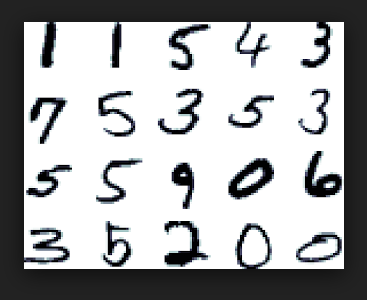
\includegraphics[width= 4.0in]{../images/MNIST}}
  
\slide{Multiclass Classification}

Assume a population distribution on pairs $(x,y)$ for $x \in \reals^d$ and $y \in \{y_1,\ldots, y_k\}$.

\vfill
For MNIST $x$ is a $28 \times 28$ image which we take to be a 784 dimensional vector giving $x \in \reals^{784}$.

\vfill
For MNIST $k = 10$.

\vfill
Let $\mathrm{Train}$ be a sample $(x_0,y_0),\;\ldots,\;(x_{N-1},y_{N-1})$ drawn IID from the population.

\slide{Multi Layer Perceptrons (MLPs)}

Activation functions:

\vfill
$$\sigma(u) = \frac{1}{1+e^{-u}}\;\;\;\;\;\;\;\;\mathrm{ReLU}(u) = \max(u,0)$$

\vfill
\centerline{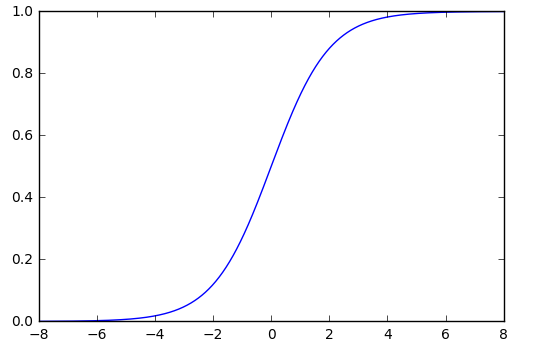
\includegraphics[width=1.5in]{../images/sigmoid}\hspace{1.0in}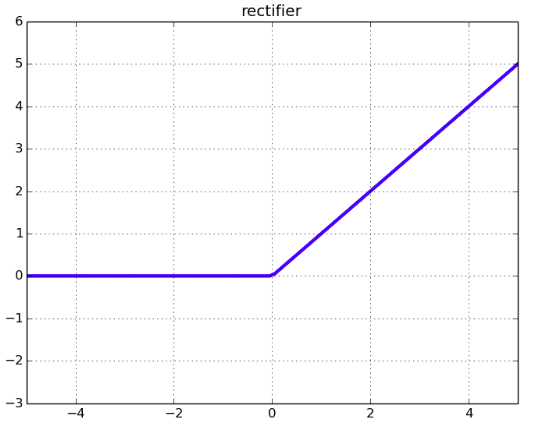
\includegraphics[width=1.2in]{../images/relu}}

\slide{An MLP in Einstein Notation (Explicit Indices)}

\centerline{$i$ --- input feature \hspace{1em} $j$ --- hidden layer feature \hspace{1em} $\hat{y}$ --- possible label}
$$\Phi = (W^0[j,i],\;b^0[j],\;W^1[\hat{y},j],\;b^1[\hat{y}])$$

\vfill
\begin{eqnarray*}
  h[j] & = & \mathrm{ReLU}\left(\left(\sum_i\;W^0[j,i] \;x[i]\right) + b^0[j]\right) \\
  \\
  s[\hat{y}] & = & \sigma\left(\left(\sum_j\;W^1[\hat{y},j]\;h[j]\right) + b^1[\hat{y}]\right) \\
  \\
  P_\Phi(\hat{y}) & = & \softmax_{\hat{y}}\;s[\hat{y}]
\end{eqnarray*}

\slide{Optimization}

Once we have specified our model $P_\Phi(y|x)$ in high level equations (such as on the previous two slides) we need to train it.

$$\Phi^* \approx \argmin_\Phi E_{(x,y) \sim \mathrm{Train}} \; {\cal L}(x,y,\Phi).$$

\vfill
The framework generates the training code automatically from the model definition.

\vfill
Optimization is almost always done with some form of stochastic gradient descent (SGD) and the gradient is computed
by back-propagation on the model definition.


\slide{Gradients with Respect to Systems of Parameters}

$\nabla_\Phi\;{\cal L}(x,y,\Phi)$ denotes the partial derivative of ${\cal L}(x,y,\Phi)$ with respect to the parameter system $\Phi$.

\vfill
We can think of $\Phi$ as a single vector with
$$(\nabla_\Phi \;{\cal L}(x,y,\Phi)\;)[i] = \partial {\cal L}(x,y,\Phi) /\partial \Phi[i]$$

\vfill
But typically $\Phi$ is actually some system of multi-dimensional arrays (tensors).

\vfill
$$\Phi = (W^0[j,i],b^0[j],W^1[\hat{y},j],b^1[\hat{y}]).$$

\vfill
$$\nabla_\Phi \;{\cal L}(x,y,\Phi) = (W^0.\mathrm{grad}[j,i],\;b^0.\mathrm{grad}[j],\;W^1.\mathrm{grad}[\hat{y},j],\;b^1.\mathrm{grad}[\hat{y}]).$$

\slide{Total Gradient Descent}

$${\cal L}_{\mathrm{Train}}(\Phi) = \frac{1}{N}\sum_n {\cal L}(\Phi,x_n,y_n)$$

\vfill
\centerline{We want: \hspace{3ex} $\Phi^*  =  \argmin_\Phi {\cal L}_{\mathrm{Train}}(\Phi)$}

\vfill
$$\Phi \;\;\;\mbox{\tt -=}\;\;\; \eta \nabla_\Phi {\cal L}_\mathrm{Train}(\Phi)$$

\slide{Stochastic Gradient Descent (SGD)}
$$\Phi^* = \argmin_\Phi E_{(x,y) \sim \mathrm{Train}} \; {\cal L}(x,y,\Phi).$$

\vfill
\begin{enumerate}
\item Randomly Initialize $\Phi$ (initialization is important and must be done with care).

  \vfill
  \item Repeat until ``converged'':

    \vfill
    \begin{itemize}
    \item draw $(x,y) \sim \mathrm{Train}$ at random.
      \vfill
    \item $\Phi \;\;\minuseq\;\; \eta \nabla_\Phi\;{\cal L}(x,y,\Phi)$
    \end{itemize}
\end{enumerate}

\slide{Stochastic Gradient Descent (SGD) on the Training set.}

\vfill
\vfill
repeat:  Select $n$ at random. $\Phi \;\;\minuseq\;\; \eta \;\nabla_\Phi \; {\cal L}(x_n,y_n,\Phi)$

\begin{eqnarray*}
  \expectsub{n}{\nabla_\Phi \; {\cal L}(x_n,y_n,\Phi)} & = & \sum_n P(n) \nabla_\Phi\;{\cal L}_{\mathrm{Train}}(x_n,y_n,\Phi) \\
  \\
  \\ & = & \frac{1}{N} \sum_n \nabla_\Phi\;{\cal L}_{\mathrm{Train}}(x_n,y_n,\Phi) \\
  \\
    \\ & = & \nabla_\Phi \frac{1}{N} \sum_n \;{\cal L}_{\mathrm{Train}}(x_n,y_n,\Phi) \\
  \\
  &  = & \nabla_\Phi\;{\cal L}_{\mathrm{Train}}(\Phi)
\end{eqnarray*}



\slide{Epochs}

In practice we cycle through the training data visiting each training pair once.

\vfill
One pass through the training data is called an Epoch.

\vfill
One typically imposes a random suffle of the training data before each epoch.

\slide{SGD for MLPs}

\centerline{$i$ --- input feature \hspace{4ex} $j$ --- hidden feature \hspace{4ex} $\hat{y}$ --- possible label}
\vfill
\centerline{$\Phi = (W^0[j,i],\;b^0[j],\;W^1[\hat{y},j],\;b^1[\hat{y}])$}

\vfill
\begin{eqnarray*}
  h[j] & = & \mathrm{ReLU}\left(\left(\sum_i\;W^0[j,i] \;x[i]\right) + b^0[j]\right) \\
  \\
  s[\hat{y}] & = & \sigma\left(\left(\sum_j\;W^1[\hat{y},j]\;h[j]\right) + b^1[\hat{y}]\right) \\
  \\
  P_\Phi(\hat{y}) & = & \softmax_{\hat{y}}\;s[\hat{y}]
\end{eqnarray*}

\vfill
We now need to automatically compute $\nabla_\Phi {\cal L}(x,y,\Phi)$.

\slide{Computation Graphs}

A computation graph (sometimes called a ``computation{\color{red} al} graph'') is a sequence of assignment statements.

\vfill
$${\cal L} = \sqrt{x^2 + y^2}$$

\vfill
Can be written as the assignment sequence:

\vfill
\begin{eqnarray*}
  u & = & x^2  \\
  v & = & y^2 \\
  r & =& u + v \\
  {\cal L} & = & \sqrt{r}
\end{eqnarray*}

\anaslide{Computation Graphs}
\vspace{-1ex}
$$\begin{array}{lcl}
 1.\;u & = & x^2  \\
 2.\;w & = & y^2 \\
 3.\;r & =& u + w \\
  4.\;{\cal L} & = & \sqrt{r}
\end{array}$$

\vfill
For each variable $z$ we can consider $\partial {\cal L}/\partial z$.

\vfill
Gradients are computed in the reverse order.

\vfill
$$\begin{array}{lcl}
(4)\; \partial{\cal L}/\partial r & = & \frac{1}{2\sqrt{r}} \\
(3)\; \partial{\cal L}/\partial u & = & \partial {\cal L}/\partial r \\
(3)\; \partial{\cal L}/\partial w & = & \partial {\cal L}/\partial r\\
(2)\; \partial{\cal L}/\partial y & = & (\partial {\cal L}/\partial w) * (2y) \\
(1)\; \partial{\cal L}/\partial x & = & (\partial {\cal L}/\partial u) * (2x)
\end{array}$$

\anaslide{A More Abstract Example}
\vspace{-3ex}
\begin{eqnarray*}
  y & = & f(x) \\
  z & = & g(y,x) \\
  u & = & h(z) \\
  {\cal L} & = & u
\end{eqnarray*}

\medskip
For now assume all values are scalars.

\medskip
We will ``backpopagate'' the assignments the reverse order.

\anaslide{Backpropagation}
\vspace{-3ex}
\begin{eqnarray*}
  y & = & f(x) \\
  z & = & g(y,x) \\
  u & = & h(z) \\
  {\cal L} &  = & {\color{red} u}
\end{eqnarray*}

\medskip
{\color{red} ${\partial {\cal L}}/{\partial u} = 1$}

\anaslide{Backpropagation}
\vspace{-3ex}
\begin{eqnarray*}
  y & = & f(x) \\
  z & = & g(y,x) \\
  u & = & h({\color{red} z}) \\
  {\cal L} &  = &  u
\end{eqnarray*}

\medskip
${\partial {\cal L}}/{\partial u} = 1$

\medskip
{\color{red} ${\partial {\cal L}}/{\partial z} = ({\partial {\cal L}}/{\partial u})\; ({\partial h}/{\partial z})$} (this uses the value of $z$)

\anaslide{Backpropagation}
\vspace{-3ex}
\begin{eqnarray*}
  y & = & f(x) \\
  z & = & g({\color{red} y},x) \\
  u & = & h(z) \\
  {\cal L} &  = &  u
\end{eqnarray*}

\medskip
${\partial {\cal L}}/{\partial u} = 1$

\medskip
${\partial {\cal L}}/{\partial z} = ({\partial {\cal L}}/{\partial u})\; ({\partial h}/{\partial z})$

\medskip
{\color{red} ${\partial {\cal L}}/{\partial y} = ({\partial {\cal L}}/{\partial z})\; ({\partial g}/{\partial y})$} (this uses the value of $y$ and $x$)

\anaslide{Backpropagation}
\vspace{-3ex}
\begin{eqnarray*}
  y & = & f({\color{red} x}) \\
  z & = & g(y,{\color{red} x}) \\
  u & = & h(z) \\
  {\cal L} &  = &  u
\end{eqnarray*}

\medskip
${\partial {\cal L}}/{\partial u} = 1$

\medskip
${\partial {\cal L}}/{\partial z} = ({\partial {\cal L}}/{\partial u})\; ({\partial h}/{\partial z})$

\medskip
${\partial {\cal L}}/{\partial y} = ({\partial {\cal L}}/{\partial z})\; ({\partial g}/{\partial y})$

\medskip
{\color{red} ${\partial {\cal L}}/{\partial x} =$ ???} Oops, we need to add up multiple occurrences.

\anaslide{Backpropagation}
\vspace{-3ex}
\begin{eqnarray*}
  y & = & f({\color{red} x}) \\
  z & = & g(y,{\color{red} x}) \\
  u & = & h(z) \\
  {\cal L} &  = &  u
\end{eqnarray*}

\medskip
We let {\color{red} $x.\grad$} be an attribute (as in Python) of node {\color{red} $x$}.

\bigskip
\bigskip
We will initialize {\color{red} $x.\mathrm{grad}$} to zero.

\bigskip
\bigskip
During backpropagation we will accumulate contributions to {\color{red} ${\partial {\cal L}}/{\partial x}$} into {\color{red} $x.\grad$}.


\anaslide{Backpropagation}
\vspace{-3ex}
\begin{eqnarray*}
  y & = & f(x) \\
  z & = & g(y,x) \\
  u & = & h(z) \\
  {\color{red} {\cal L}} &  {\color{red} =} & {\color{red}  u}
\end{eqnarray*}


\medskip
$z.\grad = y.\grad = x.\grad = 0$

\medskip
$u.\grad = 1$

\medskip
{\bf Loop Invariant}: For any variable $w$ whose definition has not yet been processed we have that $w.\grad$ is $\partial {\cal L}/\partial w$ as defined by the set of assignments already processed.

\anaslide{Backpropagation}
\vspace{-3ex}
\begin{eqnarray*}
  y & = & f(x) \\
  z & = & g(y,x) \\
  {\color{red} u} & {\color{red} =} & {\color{red} h(z)} \\
  {\color{red} {\cal L}} & {\color{red}  =} &  {\color{red} u}
\end{eqnarray*}

\medskip
$z.\grad = y.\grad = x.\grad = 0$

\medskip
$u.\grad = 1$

\medskip
{\bf Loop Invariant}: For any variable $w$ whose definition has not yet been processed we have that $w.\grad$ is $\partial {\cal L}/\partial w$ as defined by the set of assignments already processed.

\medskip
$z.\grad\;\pluseq\; u.\grad * {\partial h}/{\partial z}$

\anaslide{Backpropagation}
\vspace{-3ex}
\begin{eqnarray*}
  y & = & f(x) \\
  {\color{red} z} & {\color{red} =} & {\color{red} g(y,x)} \\
  {\color{red} u} & {\color{red} =} & {\color{red} h(z)} \\
  {\color{red} {\cal L}} & {\color{red} =} & {\color{red}  u}
\end{eqnarray*}

\medskip
$z.\grad = y.\grad = x.\grad = 0$

\medskip
$u.\grad = 1$

\medskip
    {\bf Loop Invariant}: For any variable $w$ whose definition has not yet been processed we have that $w.\grad$ is $\partial {\cal L}/\partial w$ as defined by the set of assignments already processed.

\medskip
$z.\grad\;\pluseq\; u.\grad * {\partial h}/{\partial z}$

\medskip
$y.\grad \;\pluseq\; z.\grad * {\partial g}/{\partial y}$

\medskip
$x.\grad \;\pluseq\; z.\grad * {\partial g}/{\partial x}$

\anaslideplain{Backpropagation}
\vspace{-3ex}
\begin{eqnarray*}
  {\color{red} y} & {\color{red} =} & {\color{red} f(x)} \\
  {\color{red} z} & {\color{red} =} & {\color{red} g(y,x)} \\
  {\color{red} u} & {\color{red} =} & {\color{red} h(z)} \\
  {\color{red} {\cal L}} & {\color{red} =} & {\color{red} u}
\end{eqnarray*}

\medskip
$z.\grad = y.\grad = x.\grad = 0$

\medskip
$u.\grad = 1$

\medskip
$z.\grad\;\pluseq\; u.\grad * {\partial h}/{\partial z}$

\medskip
$y.\grad \;\pluseq\; z.\grad * {\partial g}/{\partial y}$

\medskip
$x.\grad \;\pluseq\; z.\grad * {\partial g}/{\partial x}$

\medskip
$x.\grad \;\pluseq\; y.\grad * {\partial f}/{\partial x}$


\anaslide{The Vector-Valued Case}
\vspace{-3ex}
\begin{eqnarray*}
  y & = & f(x) \\
  z & = & g(y,x) \\
  u & = & h(z) \\
  {\cal L} & = & u
\end{eqnarray*}

\vfill
Now suppose the variables can be  vector-valued.

\vfill
The loss ${\cal L}$ is still a scalar.

\vfill
In this case
$$x.\mathrm{grad} = \nabla_x\;{\cal L}$$

\vfill
These are now vectors of the same dimension with
$$x.\mathrm{grad}[i] = \partial {\cal L}/\partial x[i]$$

\anaslide{The Vector-Valued Case}

$$y = f(x)$$

\vfill

In this case we consider the Jacobian matrix of $f$.

$$(\nabla_x f(x))[j,i] = \frac{\partial f(x)[j]}{\partial x[i]}$$

\vfill
We then have
$$x.\mathrm{grad}[i]\;\; \pluseq \;\; \sum_j\;y.\mathrm{grad}[j] (\nabla_x f(x))[j,i]$$


\slide{Minibatching}

Training time is greatly improved by minibatching.

 \vfill
{\bf Minibatching}: We run some number of instances together (or in parallel) and then do a parameter update based on the average
gradients of the instances of the batch.

\vfill
For NumPy minibatching is not so much about parallelism as about making the vector operations larger so that the vector operations dominate
the slowness of Python.  On a GPU minibatching allows parallelism over the batch elements.
\vfill

\slide{Minibatching}
\vfill
With minibatching each input value and each computed value is actually a batch of values.

\vfill
We add a batch index as an additional first tensor dimension for each input and computed node.

\vfill
For example, if a given input is a $D$-dimensional vector then the value of an input node
has shape $(B,D)$ where $B$ is size of the minibatch.

\vfill
Parameters do not have a batch index.

\slide{Minibatching for MLPs}

{\huge
\centerline{$b$ --- batch index \hspace{1ex} $i$ --- input feature index}
\centerline{$j$ --- hidden feature index \hspace{1ex} $\hat{y}$ --- label index}
\vfill
\centerline{$\Phi = (W^0[j,i],\;b^0[j],\;W^1[\hat{y},j],\;b^1[\hat{y}])$}
}

\vfill
\begin{eqnarray*}
  h[b,j] & = & \mathrm{ReLU}\left(\left(\sum_i\;W^0[j,i] \;x[b,i]\right) + b^0[j]\right) \\
  \\
  s[b,\hat{y}] & = & \sigma\left(\left(\sum_j\;W^1[\hat{y},j]\;h[b,j]\right) + b^1[\hat{y}]\right) \\
  \\
  P[b,\hat{y}] & = & \softmax_{\hat{y}}\;s[b,\hat{y}] \\
  \\
  {\cal L}[b] & = & - \log P[b,y[b]]
\end{eqnarray*}

\slideplain{BackProp for MLPs}

\begin{eqnarray*}
  \tilde{s}[b,\hat{y}] & = & \left(\sum_j\;W^1[\hat{y},j]\;h[b,j]\right) + b^1[\hat{y}] \\
  \\
  \\
  s[b,\hat{y}] & = & \sigma(\tilde{s}[b,\hat{y}]) \\
  \\
  \\
  \tilde{s}.\mathrm{grad}[b,\hat{y}] & \pluseq & s.\mathrm{grad}[b,\hat{y}]\;\; \sigma'|_{\tilde{s}[b,\hat{y}]}
\end{eqnarray*}

\slide{BackProp for MLPs}
\vspace{-3ex}
\begin{eqnarray*}
  \tilde{s}[b,\hat{y}] & = & \left(\sum_j\;W^1[\hat{y},j]\;h[b,j]\right) + b^1[\hat{y}] \\
  \\
  \\
  h.\mathrm{grad}[b,j] & \pluseq & \sum_{\hat{y}}\;\tilde{s}.\mathrm{grad}[b,\hat{y}]W^1[\hat{y},j] \\
  \\
  b^1.\mathrm{grad}[\hat{y}] & \pluseq & \frac{1}{B}\;\sum_b \;\tilde{s}.\mathrm{grad}[b,\hat{y}] \\
  \\
  W^1.\mathrm{grad}[\hat{y},j] & \pluseq & \frac{1}{B} \sum_b\;\tilde{s}.\mathrm{grad}[b,\hat{y}]h[b,j]
\end{eqnarray*}

By convention parameter gradients are averaged over the batch.

\slide{The Swap Rule}
\vspace{-3ex}
\begin{eqnarray*}
  \tilde{s}[b,\hat{y}] & = & \left(\sum_j\;W^1[\hat{y},j]\;h[b,j]\right) + \ldots \\
  \\
  \\
  h.\mathrm{grad}[b,j] & \pluseq & \sum_{\hat{y}}\;\tilde{s}.\mathrm{grad}[b,\hat{y}]W^1[\hat{y},j] \\
  \\
  W^1.\mathrm{grad}[\hat{y},j] & \pluseq & \frac{1}{B} \sum_b\;\tilde{s}.\mathrm{grad}[b,\hat{y}]h[b,j]
\end{eqnarray*}

When writing a backprop rule for a contraction of tensors one swaps the output with one of the inputs.

\slide{END}
}
\end{document}
